\subsection{Datenbankentwurf}
\label{sec:Datenbankentwurf}

Aufbauend auf den vorangegangenen Entwurfsergebnissen wird im Folgenden ein
Entwurf der Datenbank in Form eines Tabellenmodells angefertigt.\footnote{Ein
Tabellenmodell ist ein graphisches Modell zur Darstellung der Struktur einer
Datenbank. In diesem Modell werden Tabellen, deren Attribute (Eigenschaften)
und die Beziehung zu anderen Tabellen dargestellt.}

Bevor das Tabellenmodell erstellt werden kann, müssen in dem vorliegenden
Projekt die Daten identifiziert werden, die persistent in der Datenbank
gespeichert werden. Aus dem vorausgegangenen Oberflächenentwurf wird deutlich,
dass das Projekt aus den zwei Teilen, Benutzeransicht und Administrationsansicht,
besteht. Die Benutzeransicht stellt dabei Informationen dar, die in der
Administrationsansicht gepflegt und hinterlegt wurden. Der
Administrationsbereich ist der datenhaltende Bereich, in dem die Interaktion
mit der Datenbank stattfindet. Aus dem \verweis{Administrationsbereich} ergeben
sich bereits folgende drei Informationsobjekte:

\begin{itemize}
  \item Infotexte
  \item Fotos
  \item Interessante Orte
\end{itemize}

Die Beziehung zwischen Infotexten und Fotos stellt dabei eine sogenannte
n:m Beziehung dar. In dieser Beziehung kann ein Infotext mehreren Fotos
zugeordnet sein und im Gegenzug können ebenso mehrere Infotexte auf demselben
Foto platziert werden. Um eine solche Beziehung in einer relationalen Datenbank
abbilden zu können muss eine neue Tabelle angelegt werden, die diese Beziehung
zwischen Foto und Infotext speichert. Gleiches gilt für die
Nachbarschaftsbeziehung zwischen zwei Fotos. Da ein Foto mehrere Nachbarfotos
haben kann, muss wiederum eine Tabelle erstellt werden, in der die Beziehung
zwischen Foto und Nachbarfoto gespeichert wird. Neben diesen zwei zusätzlichen
Tabellen werden noch drei weitere Tabellen für die Speicherung der Daten der
Übersichtskarte benötigt. In der Übersichtskarte soll grundsätzlich zwischen dem
Studienstandort an der Baccumer Straße und dem Standort an der Kaiserstraße
unterschieden werden. Da beide Standorte unterschiedlich parametresiert werden 
müssen wird hierfür eine eigene Tabelle benötigt. Diese wird mit dem Namen
\textit{Area} bezeichnet. Eine Area beschreibt hierbei einen topologischen
Ausschnitt einer Google Maps Karte. Da eine topologische Karte nur den Umriss
von Gebäuden zeigt, ist es schwer, den genauen Standort eines Panoramas zu
bestimmen. Aus diesem Grund werden Grafiken über die Karte gelegt, die die
innere Struktur (Wände, Gebäudetrackte, etc.) des Campus zeigen. Sowohl die
topologische Karte als auch die übergelegten Grafiken, im folgenden
\textit{Overlays} genannt, benötigen eine eigene Tabelle, da beide jeweils noch
weitere Attribute haben. Ein Overlay ist dabei immer einer Karte zugeordnet.
Eine Karte kann weiterhin mehrere Overlays besitzen. Über die Zuordnung von
mehreren Overlays zu einer Karte werden Stockwerke an einem Standort
dargestellt. Ein Overlay enthält damit unter anderem den Pfad zu einer Grafik,
die ein Stockwerk an einem Standort darstellt. Zusammengefasst ergeben sich
folgende Tabellen:

\begin{itemize}
  \item infotext (Verwaltung der Infotexte)
  \item panorama (Verwaltung der Fotos)
  \item poi (Verwaltung der interessanten Orte)
  \item infotext\_panorama (n:m-Beziehung zwischen Infotexten und Fotos)
  \item neighbour (n:m-Beziehung zwischen zwei Fotos)
  \item area (Kartenbereich)
  \item map (Kartenansicht)
  \item overlay (übergelegte Grafik)
\end{itemize}

Diese Tabellen werden in \abbildung{Tabellenmodell} mit ihren jeweiligen
Attributen und Beziehungen dargestellt.

\begin{figure}[htb]
\centering
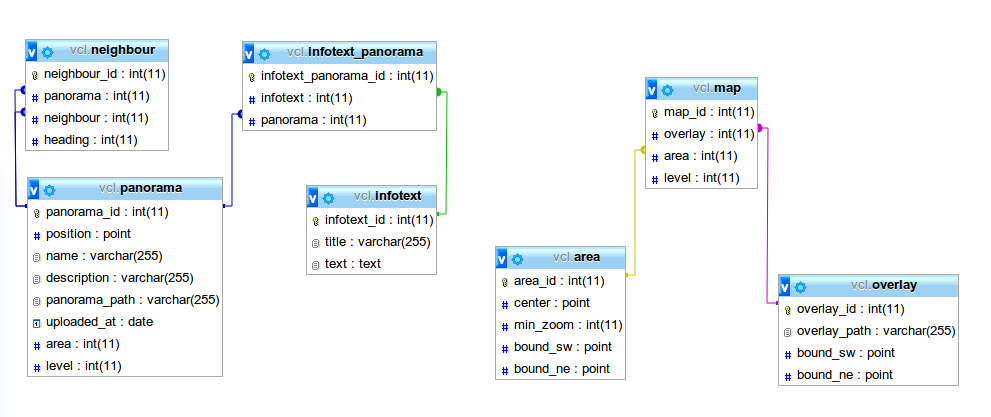
\includegraphics[width=1.0\textwidth]{Tabellenmodell.png}
\caption[Tabellenmodell der Anwendung]{Tabellenmodell der Anwendung\protect\footnotemark}
\label{fig:Tabellenmodell}
\end{figure}
\footnotetext{Quelle: Eigene Darstellung}